\documentclass[11pt, a4paper, norsk]{NTNUoving}
\usepackage[utf8]{inputenc}
\usepackage[T1]{fontenc}
\usepackage{tikz}

\ovingnr{1}    % Nummer på innlevering
\semester{Høsten 2019}
\fag{TMA 4110}
\institutt{Institutt for matematiske fag}

\begin{document}

% Kommentar

% Et felt starter ofte med \begin{<sett in kommando>}, da er det viktig å avslutte med \end{<sett in kommando>}. Det er mange eksempler på dette nedenfor!

% Du må alltid bruke $<sett inn matematikk>$, $$<sett inn matematikk>$$ eller \[<sett inn matematikk>\] for å bruke mattekommandoer.

%Dette er for enkel copy-pasting
\ifx
\begin{oppgave}
    \begin{punkt}
        \begin{align*}
        
        
        \end{align*}
    \end{punkt}
\end{oppgave}

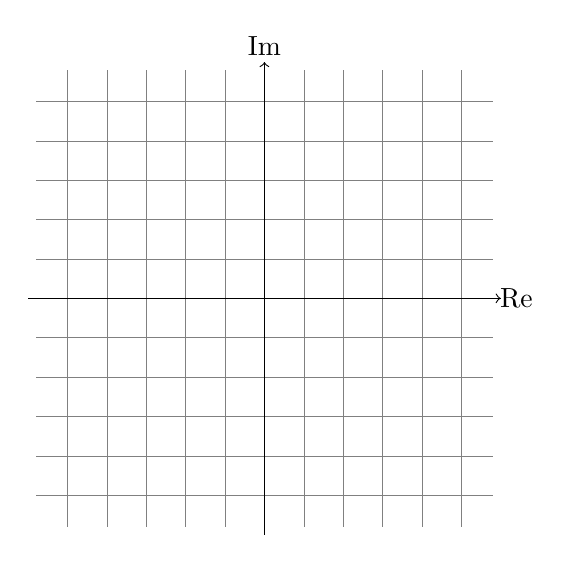
\begin{tikzpicture}
    \draw[step=.5cm,gray,very thin] (-2.9,-2.9) grid (2.9, 2.9);
    \draw (-3,0) -- (3,0);
    \draw (0,-3) -- (0,3);
    \draw[->] (-3,0) -- (3,0); 
    \draw[->] (0,-3) -- (0,3);
    \draw (0, 3.2) node {Im};
    \draw (3.2, 0) node {Re};
\end{tikzpicture}

\fi
%Her begynner dokumentet
%#####################################

\begin{oppgave}
    \begin{punkt}
        \begin{align*}
            (\sqrt{3} + i)\cdot (1-i) &= 
            \sqrt{\sqrt{3}^2 + 1^2} e^{i\arctan{\frac{1}{\sqrt{3}}}}\cdot \sqrt{1^2+(-1)^2} e^{\arctan{i\frac{-1}{1}}}
            \\&= 2\sqrt{2} e^{i\frac{\pi}{6}\frac{-\pi}{4}}
            \\&= 2\sqrt{2} e^{-i\frac{1}{12}}
        \end{align*}
    \end{punkt}
    
    \begin{punkt}
        \begin{align*}
            (\sqrt{3} + i)/ (1-i) &= 
            \frac{\sqrt{\sqrt{3}^2 + 1^2} e^{i\arctan{\frac{1}{\sqrt{3}}}}}{ \sqrt{1^2+(-1)^2} e^{\arctan{i\frac{-1}{1}}}}
            \\&= \frac{2}{\sqrt{2}} e^{i (\frac{\pi}{6}-\frac{-\pi}{4})}
            \\&=\sqrt{2}e^{i\frac{5}{12}}
        \end{align*}
    \end{punkt}
\end{oppgave}

\begin{oppgave}
    \begin{punkt}
        \begin{align*}
            e^{\frac{3\pi}{4}i} - e^{-\frac{3\pi}{4}i} &=
            z-\overline{z} = 2bi
            \\&= 2\arcsin{\frac{3\pi}{4}}i
            \\&= \sqrt{2}i = \sqrt{2} e^{\frac{\pi}{2}i}
        \end{align*}
    \end{punkt}
    
    \begin{punkt}
        \begin{align*}
            e^{\frac{3\pi}{4}i} / e^{-\frac{3\pi}{4}i} &=
            e^{(\frac{3\pi}{4}- \frac{-3\pi}{4})i}
            \\&= e^{\frac{3\pi}{2}i} (=-i)
        \end{align*}
    \end{punkt}
\end{oppgave}

\begin{oppgave}
    \begin{punkt}
        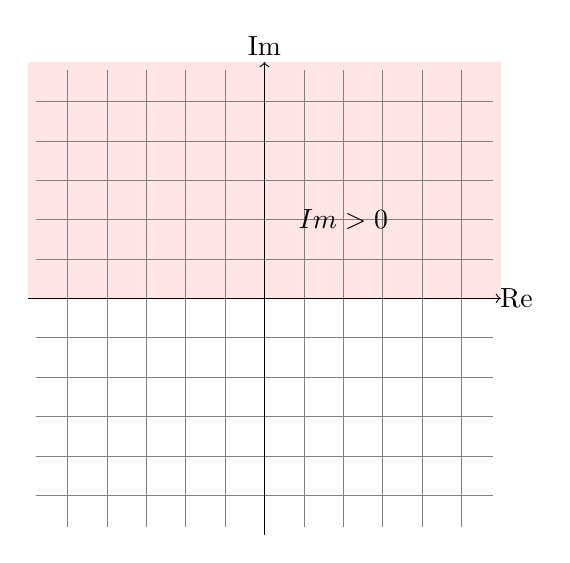
\begin{tikzpicture}
            \filldraw[red!10] (-3, 0) rectangle (3, 3);
                    
            \draw[step=.5cm,gray,very thin] (-2.9,-2.9) grid (2.9, 2.9);
            \draw (-3,0) -- (3,0);
            \draw (0,-3) -- (0,3);
            \draw[->] (-3,0) -- (3,0); 
            \draw[->] (0,-3) -- (0,3);
            \draw (0, 3.2) node {Im};
            \draw (3.2, 0) node {Re};
            \draw (1, 1) node {$Im>0$};
        \end{tikzpicture}
    \end{punkt}
    
    \begin{punkt}
        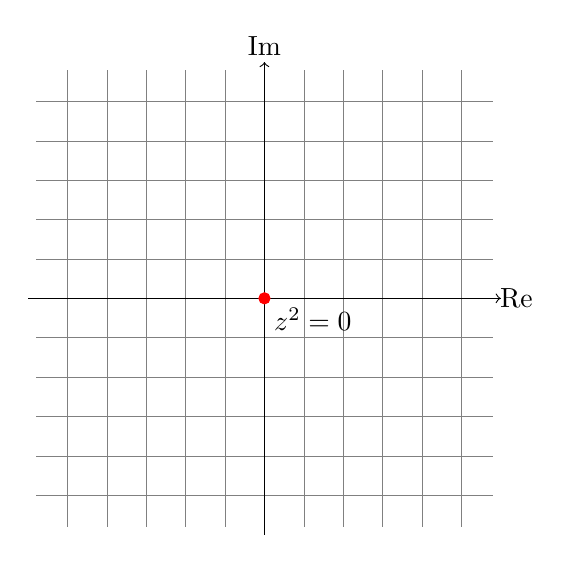
\begin{tikzpicture}
            \draw[step=.5cm,gray,very thin] (-2.9,-2.9) grid (2.9, 2.9);
            \draw (-3,0) -- (3,0);
            \draw (0,-3) -- (0,3);
            \draw[->] (-3,0) -- (3,0); 
            \draw[->] (0,-3) -- (0,3);
            \draw (0, 3.2) node {Im};
            \draw (3.2, 0) node {Re};
            \filldraw[red] (0,0) circle (2pt) node[black, anchor=north west] {$z^2 = 0$};
        \end{tikzpicture}
    \end{punkt}
    
    \begin{punkt}
        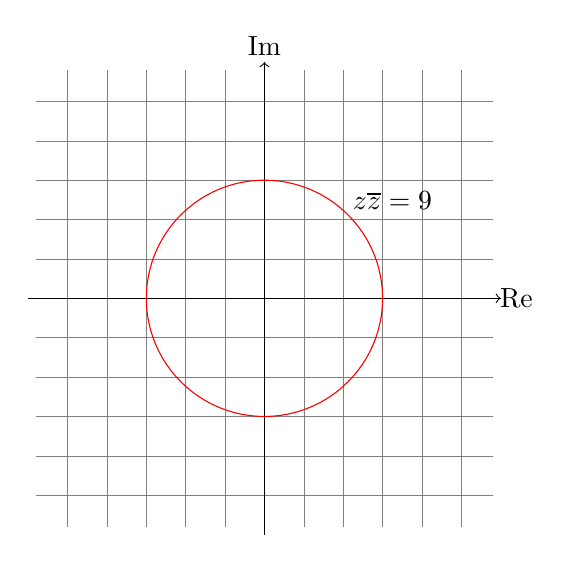
\begin{tikzpicture}
            \draw[step=.5cm,gray,very thin] (-2.9,-2.9) grid (2.9, 2.9);
            \draw (-3,0) -- (3,0);
            \draw (0,-3) -- (0,3);
            \draw[->] (-3,0) -- (3,0); 
            \draw[->] (0,-3) -- (0,3);
            \draw (0, 3.2) node {Im};
            \draw (3.2, 0) node {Re};
            
            \draw[red] (0,0) circle (1.5);
            \draw (1, 1) node[anchor=south west] {$z\overline{z} = 9$};
        \end{tikzpicture}
    \end{punkt}
    
    \begin{punkt}
        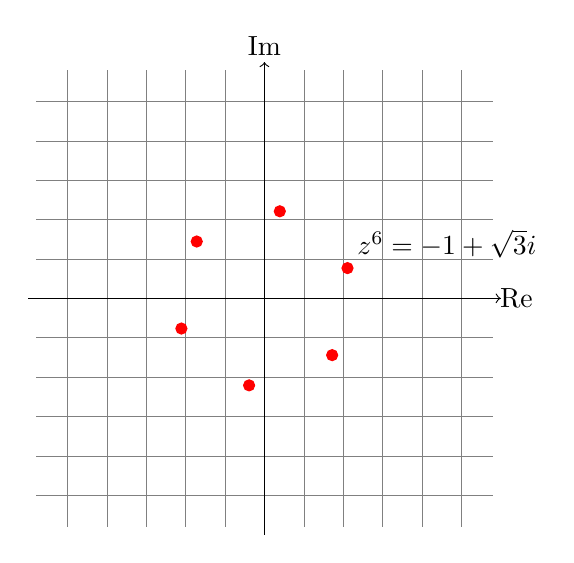
\begin{tikzpicture}
            \draw[step=.5cm,gray,very thin] (-2.9,-2.9) grid (2.9, 2.9);
            \draw (-3,0) -- (3,0);
            \draw (0,-3) -- (0,3);
            \draw[->] (-3,0) -- (3,0); 
            \draw[->] (0,-3) -- (0,3);
            \draw (0, 3.2) node {Im};
            \draw (3.2, 0) node {Re};
            \filldraw[red] (1.0547,0.3839) circle (2pt) node[black, anchor=south west] {$z^6 = -1+\sqrt{3} i$};
            \filldraw[red] (0.1949, 1.1054) circle (2pt);
            \filldraw[red] (-0.8599, 0.7215) circle (2pt);
            \filldraw[red] (-1.0547, -0.3839) circle (2pt);
            \filldraw[red] (-0.1949, -1.1054) circle (2pt);
            \filldraw[red] (0.8599, -0.7215) circle (2pt);
        \end{tikzpicture}
    \end{punkt}
    
    \begin{punkt}
        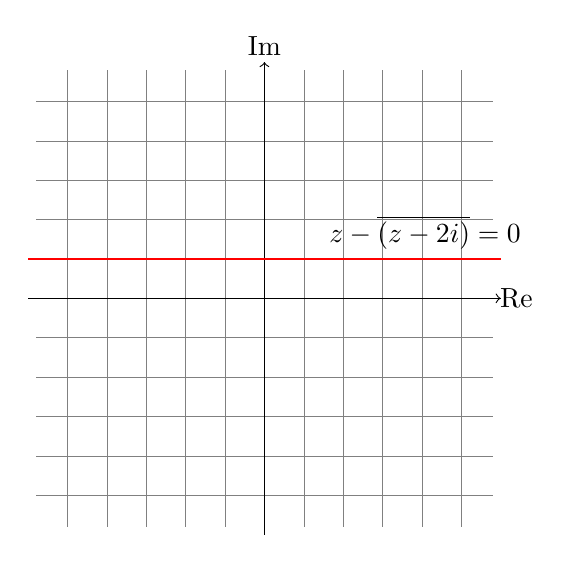
\begin{tikzpicture}
            \draw[step=.5cm,gray,very thin] (-2.9,-2.9) grid (2.9, 2.9);
            \draw (-3,0) -- (3,0);
            \draw (0,-3) -- (0,3);
            \draw[->] (-3,0) -- (3,0); 
            \draw[->] (0,-3) -- (0,3);
            \draw (0, 3.2) node {Im};
            \draw (3.2, 0) node {Re};
            
            \draw[red] (-3,0.5) -- (3, 0.5);
            \draw (0.7, 0.5) node[anchor=south west] {$z-\overline{(z-2i)} = 0$};
        \end{tikzpicture}
    \end{punkt}
\end{oppgave}

\begin{oppgave}
    \begin{punkt}
        \begin{align*}
        \overline{z/w} &= \overline{\frac{z\overline{w}}{w\overline{w}}}\\
        \\&= \frac{\overline{z}w}{w\overline{w}}\\
        \\&= \frac{\overline{z}}{\overline{w}}
        \end{align*}
    \end{punkt}
    
    \begin{punkt}
        \begin{align*}
            (\overline{z})^n &= (re^{-i\theta})^n
            \\ &= re^{-i\theta n}
            \\&= \overline{re^{i\theta n}}
            \\&= \overline{z^n}
        \end{align*}
    \end{punkt}
    
    \begin{punkt}
        \begin{align*}
            |z+w|^2 + |z-w|^2 &= |(a+c) + (b+d)i|^2 + |(a-c) + (b-d)i|^2
            \\&= (a+c)^2 + (b+d)^2 + (a-c)^2 + (b-d)^2
            \\&= a^2 + c^2 + b^2 + d^2 + a^2 + c^2 + b^2 + d^2 
            \\&= 2a^2 + 2b^2 + 2c^2 + 2d^2
            \\&= 2|z|^2 + 2|w|^2
        \end{align*}
    \end{punkt}   
    
\end{oppgave}
%###########################
%Del 2
%###########################

\begin{oppgave}[1]
    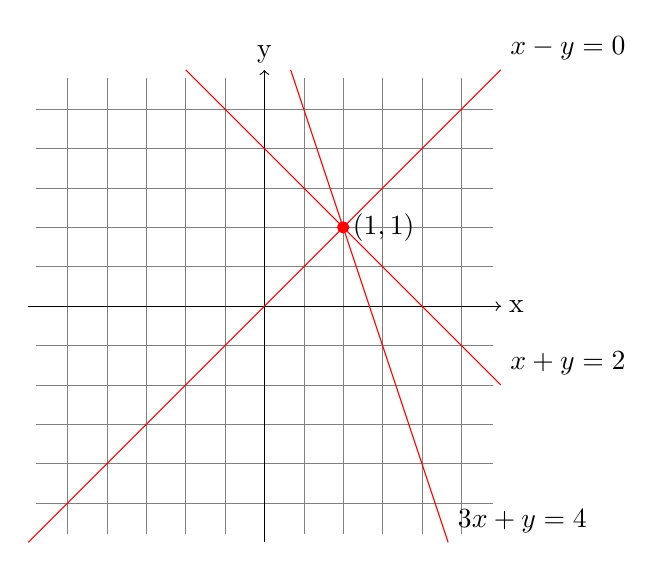
\begin{tikzpicture}
        \draw[step=.5cm,gray,very thin] (-2.9,-2.9) grid (2.9, 2.9);
        \draw (-3,0) -- (3,0);
        \draw (0,-3) -- (0,3);
        \draw[->] (-3,0) -- (3,0); 
        \draw[->] (0,-3) -- (0,3);
        \draw (0, 3.2) node {y};
        \draw (3.2, 0) node {x};
        \draw[red] (-1,3) -- (3, -1) node[black, anchor=south west]{$x+y=2$};
        \draw[red] (-3, -3) -- (3, 3) node[black, anchor=south west]{$x-y=0$};
        \draw[red] (0.3333,3) -- (2.33333, -3) node[black, anchor=south west]{$3x+y=4$};
        \filldraw[red] (1, 1) circle (2pt) node[black, anchor=west] {$(1, 1)$};
    \end{tikzpicture}
    
    Likningssettet har løsningen $x=1, y=1$.
    
\end{oppgave}

\begin{oppgave}[2]
    Ja. De to likningssystemene har den samme løsningsmengden, og de er dermed ekvivalente.
\end{oppgave}

\begin{oppgave}[3]
    Nei. Løsningsmengden til den første matrisen er $(x=1, y=0, z=0)$, mens løsningsmengden til den andre er $(x=0, y=0, z=1)$
\end{oppgave}

\begin{oppgave}[4]
    \begin{punkt}
        Nei. Her er en linje gjennom de to laveste punktene parallell med x-aksen, og siden y-komponenten til det siste punktet er ulik de to andre vil det ikke kunne ligge på samme linjen. 
    \end{punkt}
    
    \begin{punkt}
        Et polynom av grad $n$ kan entydig bestemmes fra $n+1$ punkter. Dermed finnes et andegradspolynom $f$ slik at de tre punktene ligger på  grafen til $f$. 
    \end{punkt}
\end{oppgave}

\begin{oppgave}[5]
    \begin{punkt}
        Linkingssystemet har 2 ukjente og 2 likninger. Likningene er ikke proposjonale med hverandre, eller parallelle. Da har likningssystemet én løsning. 
    \end{punkt}
    \begin{punkt}
        \begin{align*}
            \begin{cases}
            ax+by=m\\
            cx+dy=n
            \end{cases}
            \Leftrightarrow
            \begin{bmatrix} % matrise
            a & b\\
            c & d
            \end{bmatrix}
            \begin{bmatrix}
            x\\y
            \end{bmatrix}
            =
            \begin{bmatrix}
            m\\
            n
            \end{bmatrix}
        \end{align*}
        
        \begin{align*}
            \begin{bmatrix} % matrise
            a & b & m\\
            c & d & n
            \end{bmatrix}
            &\sim
            \begin{bmatrix} % matrise
            a & b & m\\
            0 & d-\frac{bc}{a} & n-\frac{mc}{a}
            \end{bmatrix}
            \\&\sim
            \begin{bmatrix} % matrise
            a & b & m\\
            0 & 1 & \frac{n-\frac{mc}{a}}{d-\frac{bc}{a}}
            \end{bmatrix}
            \\&\sim
            \begin{bmatrix}
            a & 0 & m-b\frac{n-\frac{mc}{a}}{d-\frac{bc}{a}}\\
            0 & 1 & \frac{n-\frac{mc}{a}}{d-\frac{bc}{a}}
            \end{bmatrix}
            \\&\sim
            \begin{bmatrix}
            1 & 0 & \frac{m-b\frac{n-\frac{mc}{a}}{d-\frac{bc}{a}}}{a}\\
            0 & 1 & \frac{n-\frac{mc}{a}}{d-\frac{bc}{a}}
            \end{bmatrix}
        \end{align*}
        \begin{align*}
            \\(x,y) = \left(\frac{m-b\frac{n-\frac{mc}{a}}{d-\frac{bc}{a}}}{a}, \frac{n-\frac{mc}{a}}{d-\frac{bc}{a}} \right) = \left(\frac{m}{a}-\frac{abn-bcm}{a^2d-abc}, \frac{an-mc}{ad-bc} \right)
        \end{align*}
    \end{punkt}
\end{oppgave}

\begin{oppgave}
    \begin{punkt}
        \begin{align*}
        \begin{bmatrix} % matrise
            2 & -4 & 9 & -38\\
            4 & -3 & 8 & -26\\
            -2 & 4 & -2 & 17
        \end{bmatrix}
            &\sim
        \begin{bmatrix} % matrise
            2 & -4 & 9 & -38\\
            0 & 5 & -10 & 50\\
            -2 & 4 & -2 & 17
        \end{bmatrix}
            \\&\sim
        \begin{bmatrix} % matrise
            2 & -4 & 9 & -38\\
            0 & 5 & -10 & 50\\
            0 & 0 & 7 & -21
        \end{bmatrix}
            \\&\sim
        \begin{bmatrix} % matrise
            2 & -4 & 9 & -38\\
            0 & 5 & -10 & 50\\
            0 & 0 & 1 & -3
        \end{bmatrix}
            \\&\sim
        \begin{bmatrix} % matrise
            2 & -4 & 9 & -38\\
            0 & 5 & 0 & 20\\
            0 & 0 & 1 & -3
        \end{bmatrix}
            \\&\sim
        \begin{bmatrix} % matrise
            2 & -4 & 9 & -38\\
            0 & 1 & 0 & 4\\
            0 & 0 & 1 & -3
        \end{bmatrix}
            \\&\sim
        \begin{bmatrix} % matrise
            2 & 0 & 0 & 5\\
            0 & 1 & 0 & 4\\
            0 & 0 & 1 & -3
        \end{bmatrix}
           \\&\sim
        \begin{bmatrix} % matrise
            1 & 0 & 0 & 2.5\\
            0 & 1 & 0 & 4\\
            0 & 0 & 1 & -3
        \end{bmatrix}
        \end{align*}
        \begin{align*}
        \begin{bmatrix} % matrise
            x\\
            y\\
            z
        \end{bmatrix}
        =
        \begin{bmatrix} % matrise
        2.5\\
            4\\
            -3
        \end{bmatrix}
        \end{align*}
    \end{punkt}
    
    \begin{punkt}
        \begin{align*}
        \begin{bmatrix} % matrise
            1 & 3 & 6 & 4\\
            2 & 8 & 16 & 8
        \end{bmatrix}
           &\sim
        \begin{bmatrix} % matrise
            1 & 3 & 6 & 4\\
            1 & 4 & 8 & 4
        \end{bmatrix}
           \\&\sim
        \begin{bmatrix} % matrise
            1 & 3 & 6 & 4\\
            0 & 1 & 2 & 0
        \end{bmatrix}
           \\&\sim
        \begin{bmatrix} % matrise
            1 & 3 & 6 & 4\\
            0 & 1 & 2 & 0
        \end{bmatrix}
           \\&\sim
        \begin{bmatrix} % matrise
            1 & 0 & 0 & 4\\
            0 & 1 & 2 & 0
        \end{bmatrix}
        \end{align*}
        La $y=t$, for $t \in \mathbb{R} $. Da har vi
        \begin{align*}
        \begin{bmatrix} % matrise
            x\\
            y\\
            z
        \end{bmatrix}
        =
        \begin{bmatrix} % matrise
            4\\
            t\\
            -\frac{t}{2}
        \end{bmatrix}
        \end{align*}
    \end{punkt}
    
    \begin{punkt}
    \begin{align*}
        \begin{bmatrix} % matrise
            1+i & -1 & i\\
            1-i & 1+i & 1
        \end{bmatrix}
           &\sim
        \begin{bmatrix} % matrise
            1+i & -1 & i\\
            0 & -1 & 0
        \end{bmatrix}
           \\&\sim
        \begin{bmatrix} % matrise
            1+i & -1 & i\\
            0 & 1 & 0
        \end{bmatrix}
           \\&\sim
        \begin{bmatrix} % matrise
            1+i & 0 & i\\
            0 & 1 & 0
        \end{bmatrix}
           \\&\sim
        \begin{bmatrix} % matrise
            1 & 0 & \frac{1+i}{2}\\
            0 & 1 & 0
        \end{bmatrix}
    \end{align*}
    \begin{align*}
        \begin{bmatrix} % matrise
            z\\
            w
        \end{bmatrix}
           =
        \begin{bmatrix} % matrise
            \frac{1+i}{2}\\
            0
        \end{bmatrix}
    \end{align*}
    \end{punkt}
    \begin{punkt}
        \begin{align*}
        \begin{bmatrix} % matrise
            2 & i & 5-3i & 10\\
            4 & 2i & 10+2i & 20+16i\\
            2i & -1 & 4+6i & 2 + 12i
        \end{bmatrix}
           &\sim
        \begin{bmatrix} % matrise
            2 & i & 5-3i & 10\\
            0 & 0 & 8i & 16i\\
            2i & -1 & 4+6i & 2 + 12i
        \end{bmatrix}
           \\&\sim
        \begin{bmatrix} % matrise
            2 & i & 5-3i & 10\\
            0 & 0 & 8i & 16i\\
            0 & 0 & 1+i & 2 + 2i
        \end{bmatrix}
           \\&\sim
        \begin{bmatrix} % matrise
            2 & i & 5-3i & 10\\
            0 & 0 & 1 & 2\\
            0 & 0 & 1 & 2
        \end{bmatrix}
           \\&\sim
        \begin{bmatrix} % matrise
            2 & i & 0 & 6i\\
            0 & 0 & 1 & 2\\
            0 & 0 & 0 & 0
        \end{bmatrix}
           \\&\sim
        \begin{bmatrix} % matrise
            1 & \frac{i}{2} & 0 & 3i\\
            0 & 0 & 1 & 2\\
            0 & 0 & 0 & 0
        \end{bmatrix}
        \end{align*}
        La $z=t$, for $t \in \mathbb{R}$. Da har vi
        \begin{align*}
        \begin{bmatrix} % matrise
            z\\
            w\\
            u
        \end{bmatrix}
        =
        \begin{bmatrix} % matrise
            0\\
            6\\
            2
        \end{bmatrix}
        +t
        \begin{bmatrix} % matrise
            1\\
            2i\\
            0
        \end{bmatrix}
        \end{align*}
    \end{punkt}
\end{oppgave}
\end{document}